\documentclass{article} %<<<
\usepackage{amsmath}
\usepackage{fancyvrb}
\usepackage{mathpazo}
\usepackage{microtype}
\usepackage{tikz}

\usepackage{hyperref}

\usetikzlibrary{automata,positioning,arrows}
\tikzset{automaton/.style={auto,node distance=1cm,on grid}}
\tikzset{every state/.style={minimum size=0pt,inner sep=1pt}}
\tikzset{transition/.style={->,>=stealth',shorten >=1pt}}
\tikzset{every initial by arrow/.style={transition}}
\tikzset{initial text={}}

\title{Static Checking of TOPL Properties}
\author{
  Dino Distefano
  \and Radu Grigore
  \and Rasmus Lerchedahl Petersen
  \and Nikos Tzevelekos}

%>>>
\begin{document} %>>>
\maketitle

We want to prove that a given program does not violate a given topl property.
The main idea is that almost any static analyzer is sufficient.
Why?
Well, suppose the \emph{runtime} monitor faults when a violation occurs.
If a static analyzer concludes that the instrumented program, including the monitor, cannot fault, then this means the topl property was checked statically.
The static analyzer must be able to modularly infer specifications, for example via abduction.
Otherwise the verification would be very inconvenient.

Consider the topl property
\[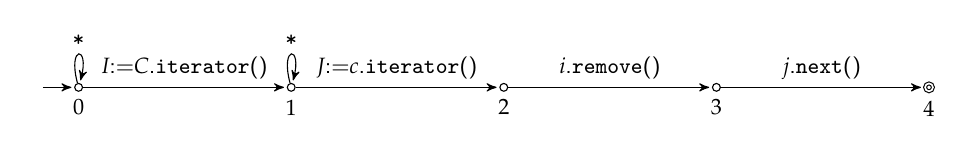
\begin{tikzpicture}[automaton,node distance=2.7cm]\footnotesize
  \node[state,initial] (q0) [label=below:$0$] {};
  \node[state] (q1) [label=below:$1$,right=of q0] {};
  \node[state] (q2) [label=below:$2$,right=of q1] {};
  \node[state] (q3) [label=below:$3$,right=of q2] {};
  \node[state,accepting] (q4) [label=below:$4$,right=of q3] {};
  \path[transition]
    (q0) edge node{{\it I}{\sf :=}{\it C}{\sf.}{\tt iterator}{\sf()}} (q1)
         edge[loop above] node{\tt*} ()
    (q1) edge node{{\it J}{\sf :=}{\it c}{\sf.}{\tt iterator}{\sf()}} (q2)
         edge[loop above] node{\tt*} ()
    (q2) edge node{{\it i}{\sf.}{\tt remove}{\sf()}} (q3)
    (q3) edge node{{\it j}{\sf .}{\tt next}{\sf()}} (q4);
\end{tikzpicture}\]
To check that a program does not violate it we run a static verifier on a modified program.
We add global variables {\tt state}, {\tt c}, {\tt i}, and~{\tt j}.
We replace calls to {\tt iterator} by calls to {\tt iterator'}, calls to {\tt remove} by calls to {\tt remove'}, and calls to {\tt next} by calls to {\tt next'}.
The primed methods are implemented as follows.
\begin{Verbatim}[fontsize=\footnotesize]
  Iterator iterator'() {
    emit(new Event(1, new Object[]{this}));
    Iterator r = iterator();
    emit(new Event(2, new Object[]{r}));
    return r;
  }
  void remove'() {
    emit(new Event(3, new Object[]{this}));
    remove();
  }
  Object next'() {
    emit(new Event(4, new Object[]{this}));
    return next();
  }
\end{Verbatim}
This is essentially the same as is done in the runtime verifier---each observable method announces when it is called and when it returns.
Each call and each return gets an \emph{event identifier} (from~$1$ to~$4$ in this example).
In this example events carry $0$~or~$1$ objects, but for other properties there might be more, which is why an array is used to store them.
The method {\tt emit} uses another global variable, the queue~$E$ of events.
\begin{Verbatim}[fontsize=\footnotesize]
  void emit(Event e) {
    E.enque(e);
    step();
  }
\end{Verbatim}
The method {\tt step} advances the configuration of the r-topl automaton, which is represented by the integer {\tt state} and the queue {\tt events}.

We should find a specification for {\tt step}.
Alternatively, the static analyzer could infer the specification from an implementation of {\tt step}.
But, of course, we cannot expect a generic specification inference heuristic to do as well as an algorithm that exploits the special structure of~{\tt step}.

The specification of {\tt step} is complex, so good notation is needed.
The queue~$E$ has bounded size~$E_{\rm sz}$.
In this example, $E_{\rm sz}$~is $0$,~$1$, or~$2$.
Each event $E_i$ contains a bounded number of values~$E_{i,j}$, and has an identifier~$E_{i,{\rm id}}$.
Thus, the queue is represented by a set of primitive global variables.
In this example the variables are $E_{\rm sz}$,~$E_{0,{\rm id}}$, $E_{0,0}$, $E_{1,{\rm id}}$, and~$E_{1,0}$.

Each state~$q$ has an associated formula which means `state $q$ is active and we know enough events to simulate one step of the automaton'
\[ P_q \quad=\quad ({\it state}=q) \land (E_{\rm sz}\ge d_q) \]
where $d_q$~is the maximum length of a transition outgoing from~$q$.
Each transition~$t$ has two associated formulas.
Its \emph{precondition} identifies the configurations in which $t$~is enabled.
\begin{multline*}
P_t \quad=\quad
    \bigl(g_0\circ(E_0:=E_0)\bigr)
    \land\bigl(g_1\circ(E_0:=E_1)\circ a_0\bigr)
    \land\ldots\\\ldots
    \land\bigl(g_{n-1}\circ (E_0:=E_{n-1})\circ a_{n-2} \circ\cdots\circ a_1\circ a_0\bigr)
\end{multline*}
Here $g_0,\ldots,g_{n-1}$ are the guards of~$t$, and $a_0,\ldots,a_{n-1}$ are its actions.
The guards are formulas to begin with, interpreted over a store~$\sigma$ and a letter~$\ell$.
In our case the store~$\sigma$ consists of a few global variables ({\tt c}, {\tt i}, {\tt j}), and the letter~$\ell$ is the oldest unprocessed event~$E_0$.
Assignments and actions are seen as substitutions, and $g\circ a$ is the formula obtained by applying the substitution~$a$ to~$g$, which can also be seen as a form of function composition.
Its \emph{postcondition} encodes the action of the transition.
\[ Q_t \quad=\quad
  ({\it state}=q')
  \land D(n)
  \land (I\circ a_{n-1}\circ\cdots\circ a_0)
  \]
The state $q'$ is the destination of~$t$.
The formula~$D(n)$ encodes dropping $n$~events from~$E$.
The formula~$I$ states that the variables $x_1$,~$x_2$, $\ldots$~that make up the store remain unchanged.
(Of course, substitutions leave ${\sf old}(\ldots)$ unchanged.)
\begin{align*}
D(n) \quad&=\quad
  \bigl(E_{\rm sz}={\sf old}(E_{\rm sz})-n\bigr)
  \land\bigl(E_0={\sf old}(E_n)\bigr)
  \land\bigl(E_1={\sf old}(E_{n+1})\bigr)
  \land\ldots\\
I \quad&=\quad
  \bigl(x_1={\sf old}(x_1)\bigr)
  \land\bigl(x_2={\sf old}(x_2)\bigr)
  \land\ldots
\end{align*}
In particular, $D(0)$~is the identity for the variables that represent the queue~$E$.
In our example the following definitions would work:
{\def\=#1{(#1={\sf old}(#1))}
\begin{align*}
D(0) \quad&=\quad \={E_{\rm sz}}\land\={E_0}\land\={E_1} \\
D(1) \quad&=\quad (E_{\rm sz}={\sf old}(E_{\rm sz})-1)\land(E_0={\sf old}(E_1)) \\
D(2) \quad&=\quad (E_{\rm sz}={\sf old}(E_{\rm sz})-2) \\
I \quad&=\quad \=c\land\=i\land\=j
\end{align*}}

Let $t_1$~and~$t_2$ be transitions outgoing from~$q$.
Let $S$ be the symbolic state just before the call to {\tt step}.
Suppose $S$ implies both $P_{t_1}$~and~$P_{t_2}$.
Intuitively this means that $t_1$~and~$t_2$ are both enabled.
After the call to {\tt step} the concrete state should satisfy $Q_{t_1}\lor Q_{t_2}$.
Nondeterminism is represented by disjunction.
(Conjunction cannot work because $({\it state}=0)\land({\it state}=1)$ is equivalent to false.)
In general, let $t_1$,~$t_2$, \dots,~$t_n$ be all the transitions outgoing from state~$q$.
Then the following are $2^{n-1}$ good contracts for {\tt step}:
\[
  \left\{\begin{aligned}
  &P_q&&\\
  &P_{t_k}  &&\text{for $k\in T$} \\
  &\lnot P_{t_k}  &&\text{for $k\notin T$}
  \end{aligned}\right\}
  \quad\text{\tt step}\quad
  \left\{\bigvee_{k\in T}Q_{t_k}\right\}
  \qquad\text{for $\emptyset\subset T\subseteq \{1,2,\ldots,n\}$}
\]
The conditions listed in the precondition are implicitly conjoined.
The set~$T$ of enabled transitions must be not empty.
Otherwise, if no outgoing transition is enabled, the contract must drop one event.
\[
  \{P_q\land\lnot P_{t_1}\land\ldots\land\lnot P_{t_n}\}
  \quad\text{\tt step}\quad
  \{({\it state}=q)\land D(1)\land I\}
\]
If the queue~$E$ does not contain sufficient events, then {\tt step} should be a no-operation.
\[
  \{({\it state}=q)\land(E_{\rm sz}<d_q)\}
  \quad\text{\tt step}\quad
  \{({\it state}=q)\land D(0)\land I\}
\]

Note that the preconditions listed so far for {\tt step} are mutually unsatisfiable.
This means that the conjunction rule of Hoare logic cannot be used.
The disjunction rule of Hoare logic, on the other hand, must be used, to handle the disjunctions that represent nondeterminism.

Let us now spell out the contract of {\tt step} in the case of the running example.
There are four no-op contracts with satisfiable preconditions:
\begin{align*}
\{({\it state}=0)\land(E_{\rm sz}<2)\} \quad\text{\tt step}\quad
  \{({\it state}=0)\land D(0)\land I\} \\
\{({\it state}=1)\land(E_{\rm sz}<2)\} \quad\text{\tt step}\quad
  \{({\it state}=1)\land D(0)\land I\} \\
\{({\it state}=2)\land(E_{\rm sz}<1)\} \quad\text{\tt step}\quad
  \{({\it state}=2)\land D(0)\land I\} \\
\{({\it state}=3)\land(E_{\rm sz}<1)\} \quad\text{\tt step}\quad
  \{({\it state}=3)\land D(0)\land I\}
\end{align*}
The most complicated state is probably $1$:
It has two outgoing transitions of different lengths, and the longer one uses both (nontrivial) guards and actions.
The loop on~$1$ has the precondition ${\it true}$ and the postcondition
\[ ({\it state}=1) \land D(1) \land I \]
The transition from~$1$ to~$2$ has the precondition
\[ (E_{0,{\rm id}}=1)\land(c=E_{0,0}) \]
which is essentially the guard of the first step, and the postcondition
\[ ({\it state}=2)\land D(2)\land E\]
TODO: Oops, the substitutions I have don't work as I wanted.



OLD:


\begin{align*}
P_1&:\left\{\begin{aligned}
    &{\it state}=0 \land E_{\rm sz}\ge2 \\
    &E_{0,{\rm id}}=1 \land E_{1,{\rm id}}=2
    \end{aligned}\right\}
  &Q_1&:\left\{\begin{aligned}
    {\it state}&=1\\
    E_{\rm sz}&=0\\
    i&={\sf old}(E_{0,0})\\
    c&={\sf old}(E_{1,0})
    \end{aligned}\right\}\\
P'_1&:\left\{\begin{aligned}
    {\it state}=0 \land E_{\rm sz}\ge2
    \end{aligned}\right\}
  &Q'_1&:\left\{\begin{aligned}
  E_{\rm sz}&=1\\
  E_0&={\sf old}(E_1)
  \end{aligned}\right\} \\
P_2&:\left\{\begin{aligned}
    &{\it state}=1 \land E_{\rm sz}\ge2\\
    &E_{0,{\rm id}}=1 \land E_{0,0}=c \land E_{1,{\rm id}}=2
    \end{aligned}\right\}
  &Q_2&:\left\{\begin{aligned}
    {\it state}&=2\\
    E_{\rm sz}&=0\\
    j&={\sf old}(E_{1,0})
    \end{aligned}\right\}\\
P_3&:\left\{\begin{aligned}
    &{\it state}=2 \land E_{\rm sz}\ge1 \\
    &E_{0,{\rm id}}=3 \land E_{0,0}=i
    \end{aligned}\right\}
  &Q_3&:\left\{\begin{aligned}
    {\it state}&=3\\
    E_{\rm sz}&={\sf old}(E_{\rm sz})-1\\
    E_0&={\sf old}(E_1)
    \end{aligned}\right\}\\
P_4&:\left\{\begin{aligned}
    &{\it state}=3 \land E_{\rm sz}\ge1\\
    &E_{0,{\rm id}}=4 \land E_{0,0}=j
    \end{aligned}\right\}
  &Q_4&:\left\{\begin{aligned}
    {\it state}&=4\\
    E_{\rm sz}&={\sf old}(E_{\rm sz})-1\\
    E_0&={\sf old}(E_1)
    \end{aligned}\right\}
\end{align*}
All global variables~$x$ that do not appear in the postcondition written above are understood to contribute the equality $x={\sf old}(x)$.
Each state of the automaton could contribute a (precondition, postcondition) pair to the specification of {\tt step}, to simulate skip configuration transitions.
\begin{align*}
P_5&:\left\{\begin{aligned}
    &{\it state}=0 \land E_{\rm sz}=2 \\
    &E_{0,{\rm id}}\ne1\lor E_{1,{\rm id}}\ne2
    \end{aligned}\right\}
  &Q_5&:\left\{\begin{aligned}
    E_{\rm sz}&=1\\
    E_0&={\sf old}(E_1)
    \end{aligned}\right\} \\
P_6&:\left\{\begin{aligned}
    &{\it state}=1 \land E_{\rm sz}=2 \\
    &E_{0,{\rm id}}\ne1\lor E_{0,0}\ne c \lor E_{1,{\rm id}}\ne2
    \end{aligned}\right\}
  &Q_6&:\left\{\begin{aligned}
    E_{\rm sz}&=1\\
    E_0&={\sf old}(E_1)
    \end{aligned}\right\}
\end{align*}
TODO: Do nothing when not enough events; Don't go to error, so proof gets stuck.

\end{document} %>>>
% vim:fmr=<<<,>>>:
